% Online sync refresh: revised workshop report, 2026-08-29. figure-path-fix
The gradient-bandit and UCB algorithms were compared on the same
10-armed bandit over \(T=10^4\) time steps and \(M=300\) independent
reruns. For each run, cumulative pseudo-regret was computed as
\[
    \sum_{t=1}^{T}
    \left[
        R^\ast-q^\ast(A_t)
    \right],
\]
and averaged across reruns. The comparison uses UCB with
\(c\in\{0,1,2\}\) and the gradient-bandit algorithm with
\(\alpha\in\{0,0.1,0.5\}\).

\begin{figure}[H]
    \centering
    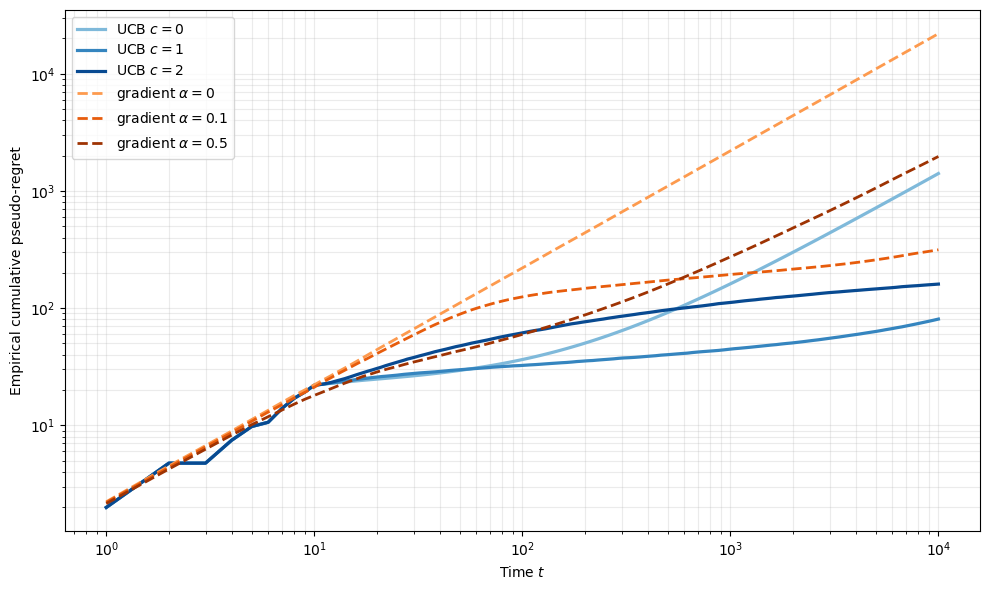
\includegraphics[width=0.76\linewidth]
    {figures/q6_gradient_vs_ucb_regret.png}
    \caption{Empirical cumulative pseudo-regret of the gradient-bandit
    and UCB algorithms over \(T=10^4\) time steps.}
    \label{fig:q6-gradient-ucb-regret}
\end{figure}

The cumulative pseudo-regret at \(T=10^4\) is summarised in
Table~\ref{tab:q6-regret}.

\begin{table}[H]
    \centering
    \caption{Empirical cumulative pseudo-regret at \(T=10^4\).}
    \label{tab:q6-regret}
    \begin{tabular}{lc}
        \toprule
        \textbf{Algorithm} & \textbf{Cumulative pseudo-regret} \\
        \midrule
        UCB, \(c=1\) & \(80.58\) \\
        UCB, \(c=2\) & \(160.29\) \\
        Gradient, \(\alpha=0.1\) & \(314.58\) \\
        UCB, \(c=0\) & \(1408.07\) \\
        Gradient, \(\alpha=0.5\) & \(1968.16\) \\
        Gradient, \(\alpha=0\) & \(21978.00\) \\
        \bottomrule
    \end{tabular}
\end{table}

Figure~\ref{fig:q6-gradient-ucb-regret} and
Table~\ref{tab:q6-regret} show that exploratory UCB achieves the lowest
regret: \(c=1\) gives \(80.58\), followed by \(c=2\) with \(160.29\).
The best gradient case, \(\alpha=0.1\), gives \(314.58\): about four times
the regret of UCB with \(c=1\), but well below non-exploratory UCB. The
larger \(\alpha=0.5\) result, \(1968.16\), shows greater sensitivity to
reward noise; with \(\alpha=0\), the policy stays uniform and regret is
approximately linear. Thus, for this instance and the tested parameters,
exploratory UCB gives the more regret-efficient trade-off.
